\documentclass{cosas/tfg_domingo}
% \documentclass[numeros]{tfg_domingo}

\autor{Alejandro Martínez Floranes}
\titulo{Reescribir slatt en Python 3}
% Título corto para los encabezamientos de pagina:
\corto{} % En blanco si no es necesario recortarlo.
\ingles{Rewrite slatt in Python 3}
\fecha{julio de 2021}
% La normativa prescribe «cuatro o cinco palabras clave, en
% español y en inglés, para su indexación en el repositorio
% de TFG».
\palabras{reglas de asociación, hipergrafos, slatt, refactorizar}%
  {association rules, hypergraph, slatt, refactor}

\usepackage{lipsum} % Esto solo es relleno.
\usepackage{listings}
\usepackage{xcolor}
\usepackage{amssymb}
\usepackage{multirow}

\definecolor{codegreen}{rgb}{0,0.6,0}
\definecolor{codegray}{rgb}{0.5,0.5,0.5}
\definecolor{codepurple}{rgb}{0.58,0,0.82}
\definecolor{backcolour}{rgb}{0.95,0.95,0.92}

\lstdefinestyle{mystyle}{
    %backgroundcolor=\color{backcolour},   
    commentstyle=\color{codegreen},
    keywordstyle=\color{magenta},
    numberstyle=\tiny\color{codegray},
    stringstyle=\color{codepurple},
    basicstyle=\ttfamily\footnotesize,
    breakatwhitespace=false,         
    breaklines=true,                 
    captionpos=b,                    
    keepspaces=true,                 
    numbers=left,                    
    numbersep=5pt,                  
    showspaces=false,                
    showstringspaces=false,
    showtabs=false,                  
    tabsize=2
}

\lstset{style=mystyle}

\begin{document}

% Si alguna palabra se divide entre dos líneas en un punto
% indebido, podemos indicar aquí los puntos de corte
% aceptables (si los hay), p. ej,
% \hyphenation{ba-rro-co, frío, cria-do, su-per-ra-tón}
\hyphenation{Dijkstra new-speak}

\portada
\frontmatter
% \sucinto{A Sofía}
\gracias{\input{cosas/agradecimientos.txt}}
\resumen{Las reglas de asociación son objetos matemáticos empleados de forma extensa en disciplinas como la minería de datos, aprendizaje automático y representación del conocimiento, entre otros campos.
Slatt es un proyecto de software libre desarrollado por José Luis Balcázar (Universidad Politécnica de Barcelona). Ofrece funcionalidades para el cálculo de reglas de asociación. Para ello, se apoya en implementaciones del algoritmo a priori para el cálculo de clausuras, el retículo de las clausuras y, entre otras
funcionalidades,devuelve las reglas representativas para cualquier elección de los parámetros de soporte y confianza.

En este proyecto, se ha mejorado este software utilizando como base las implementaciones disponibles en Slatt aplicadas a:

\begin{itemize}
    \item hipergrafos y algoritmos con aplicación a estos objetos;
    
    \item cálculo de clausuras y retículos (lattices);
\end{itemize}


Este trabajo ha requerido la búsqueda y análisis de algoritmos propuestos en la literatura científica sobre los puntos anteriores.
El lenguaje de desarrollo será Python3, encontrándose la implementación anterior en Python 2.7
%
% Conviene evitar aquí las llamadas a la bibliografía del
% trabajo, ya que el resumen tiene entidad independiente.
%

%% Aportamos nuestra perspectiva sobre la pertinencia de las
%% instrucciones {\tt goto}.


%%Pasar a tiempo presente
}{Association rules are mathematical objects used extensively in disciplines such as data mining, machine learning, and knowledge representation, among other fields.
Slatt is a free software project developed by José Luis Balcázar (Polytechnic University of Barcelona). It offers functionalities for the calculation of association rules. To do this, it relies on implementations of the a priori algorithm for the calculation of closures, the lattice of closures and, among others
functionalities, returns the representative rules for any choice of support and trust parameters.

In this project, this software has been improved using as a basis the implementations available in Slatt applied to:

\begin{itemize}
    \item hypergraphs and algorithms with application to these objects;
    
    \item calculation of closures and lattices (lattices);
\end{itemize}


This work has required the search and analysis of algorithms proposed in the scientific literature on the previous points.
The development language will be Python3, the previous implementation being in Python 2.7
}
\tableofcontents

\mainmatter
\chapter{\emph{Introducción}}

\section{Reglas de asociación}

Este proyecto se basa principalmente en reescribir \textbf{slatt} en Python 3 e incluir diferentes mejoras en el código para mejorar tanto su eficiencia en cuanto a rendimiento, como en reducción de lineas de código, y realizar una mejora en la legibilidad del propio código.

Slatt es un proyecto de software libre que ofrece funcionalidades para el cálculo de reglas de asociación. 

Las reglas de asociación son declaraciones 'if-then' que ayudan a mostrar la probabilidad de relaciones entre elementos de datos, dentro de grandes conjuntos de datos. Las medidas de evaluación  de las reglas de asociación son: \textit{el soporte, la confianza y el lift.} 

\begin{itemize}
    \item El \textbf{soporte} es la fracción de las transacciones que contiene tanto a X como a Y. 
    \item La \textbf{confianza} es la fracción de las transacciones en las que aparece X que también incluyen a Y; esto es, la confianza mide con que frecuencia aparece Y en las transacciones que incluyen X.
    \item El \textbf{lift} es la confianza de la reglas dividido por el cociente del consecuente.
\end{itemize}

\begin{figure}[ht!] % [h!] fuerza que el elemento se sitúe
                    % en la posición señalada, en vez de al
                    % comienzo de una página.
\begin{center}
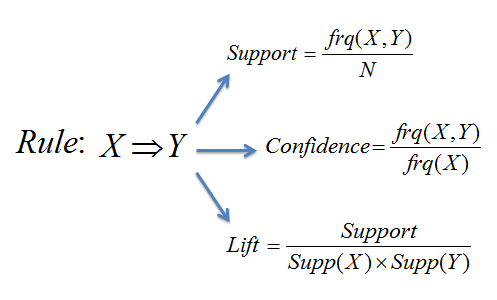
\includegraphics[width=.49\linewidth]{imagenes/AR_1.png}
\end{center}
\caption{Association Rules}
\label{fig_pro}
\end{figure}

A su vez, a la hora de plantear un problema utilizando reglas de asociación necesitamos disponer de diferentes elementos: 

\begin{enumerate}
    \item \textbf{Itemset.- }Conjunto de uno o más items (artículos).
    \item \textbf{K-itemset.- } Itemset con k elementos.
    \item \textbf{Soporte de un itemset.- } Fracción de las transacciones que contienen el itemset.
    \textbf{Itemset Frecuente} Itemset con soporte igual o superior a un umbral de soporte establecido por el usuario.
    \item \textbf{Umbral mínimo de confianza y de soporte.- } estos umbrales se utilizan para coger las reglas cuyo soporte o confianza sean mayores que las de umbral mínimo.
\end{enumerate}

Ejemplo sencillo de como utilizar las reglas de asociación para un problema general (problema de la lista de la compra). \citep{berzal2016reglas}

\begin{table}[h]
\centering
\begin{tabular}{|l|l|l|}
\hline
TID & Artículos                     \\ \hline
1         & Pan, leche, huevos            \\ \hline
2         & Pan, pañales, cerveza            \\ \hline
3         & Leche, pañales, cerveza            \\ \hline
4         & Pan, leche, pañales, cerveza         \\ \hline
5         & Pan, leche, huevos, cerveza         \\ \hline
\end{tabular}
\caption{Problema reglas de asociación}
\label{tab:my-table}
\end{table}

\begin{itemize}
    \item El \textbf{soporte} de la cerveza, supp(cerveza) = 4/5 = 0.8
    
    \item El \textbf{soporte} de los pañales, supp(pañales) = 3/5 = 0.6
    
    \item El \textbf{soporte} de la cerveza y los pañales, supp(cerveza,pañales) = 3/5 = 0.6
    
    \item La \textbf{confianza} entre la cerveza y los pañales seria, supp(cerveza,pañales) / supp(cerveza) 
   
    = 0.6 / 0.8 = 0.75
\end{itemize}

Para implementar este tipo de operaciones en código python, Slatt se basa principalmente en el algoritmo \textit{Apriori}, el proceso de este algoritmo sigue dos pasos: \citep{morales2013reglas}

\begin{enumerate}
    \item Genera los itemsets.
    \begin{itemize}
        \item Genera todos los itemsets con un elemento.
        \item Usa estos para generar los de dos elementos, y así sucesivamente.
        \item Toma todos los que cumplen con el mínimo soporte (esto permite eliminar posibles combinaciones).
    \end{itemize}
    \item Genera las reglas revisando que cumplan con el criterio mínimo de confianza.
\end{enumerate}

\lstinputlisting[language=python,caption=\textbf{Apriori Algorithm pyhton version},frame=bottom]{codigo/apriori.py}




% Utilice «citet» para integrar el nombre del autor en el
% texto. Para referencias aisladas, «citep».

\newpage
\section{Metodología y Requisitos}

Para la realización del proyecto se ha utilizado una metodología incremental, debido a que dicho proyecto esta dividido en diferentes partes, las cuales unas no tienen relación directa con otras, es por esto, que he decidió usar este tipo de metodología.

\begin{figure}[ht!] % [h!] fuerza que el elemento se sitúe
                    % en la posición señalada, en vez de al
                    % comienzo de una página.
\begin{center}
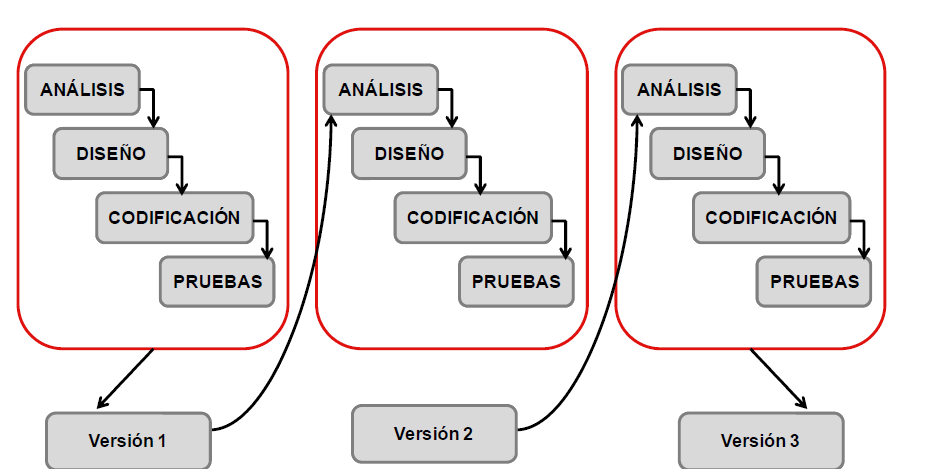
\includegraphics[width=.7\linewidth]{imagenes/Metodologia.png}
\end{center}
\caption{Metodología iterativa incremental}
\label{fig_pro}
\end{figure}

A continuación, defino los requisitos funcionales y no funcionales del proyecto software, al no ser una aplicación destinada hacia un usuario(cliente), los requisitos no funcionales, se basan en el correcto funcionamiento de la aplicación y los requisitos funcionales

\begin{table}[h]
\centering
\begin{tabular}{|l|l|}
\hline
Identificador & Descripción                     \\ \hline
RF01         & La aplicación deberá            \\ \hline
RF02         & La mejora en python3            \\ \hline
RF03         & La mejora en python3            \\ \hline
RF04         & La refactorización de l         \\ \hline
\end{tabular}
\caption{Requisitos funcionales del proyecto}
\label{tab:my-table}
\end{table}

\begin{table}[h]
\centering
\begin{tabular}{|l|l|}
\hline
Identificador & Descripción                              \\ \hline
RNF01         & La aplicación deberá tener la misma funcionalidad tanto en python2 como en python3                                          \\ \hline
RNF02          & La mejora en python3 deberá ser mas eficiente que la de su anterior versión                                                  \\ \hline
RNF03          & La mejora en python3 deberá tener menos lineas de código que su anterior versión                                         \\ \hline
RNF04          & La refactorización de los métodos no supondrá un cambio en los resultados                                               \\ \hline
\end{tabular}
\caption{Requisitos no funcionales del proyecto}
\label{tab:my-table}
\end{table}

\newpage

\section{Diagrama de clases UML}
En este apartado indico el diagrama de clases UML inicial de Slatt escrito en pyhton2 y el resultado final del proyecto al reescribirlo a python3 con las nuevas clases, herencias, etc.

\begin{figure}[ht!] % [h!] fuerza que el elemento se sitúe
                    % en la posición señalada, en vez de al
                    % comienzo de una página.
\begin{center}
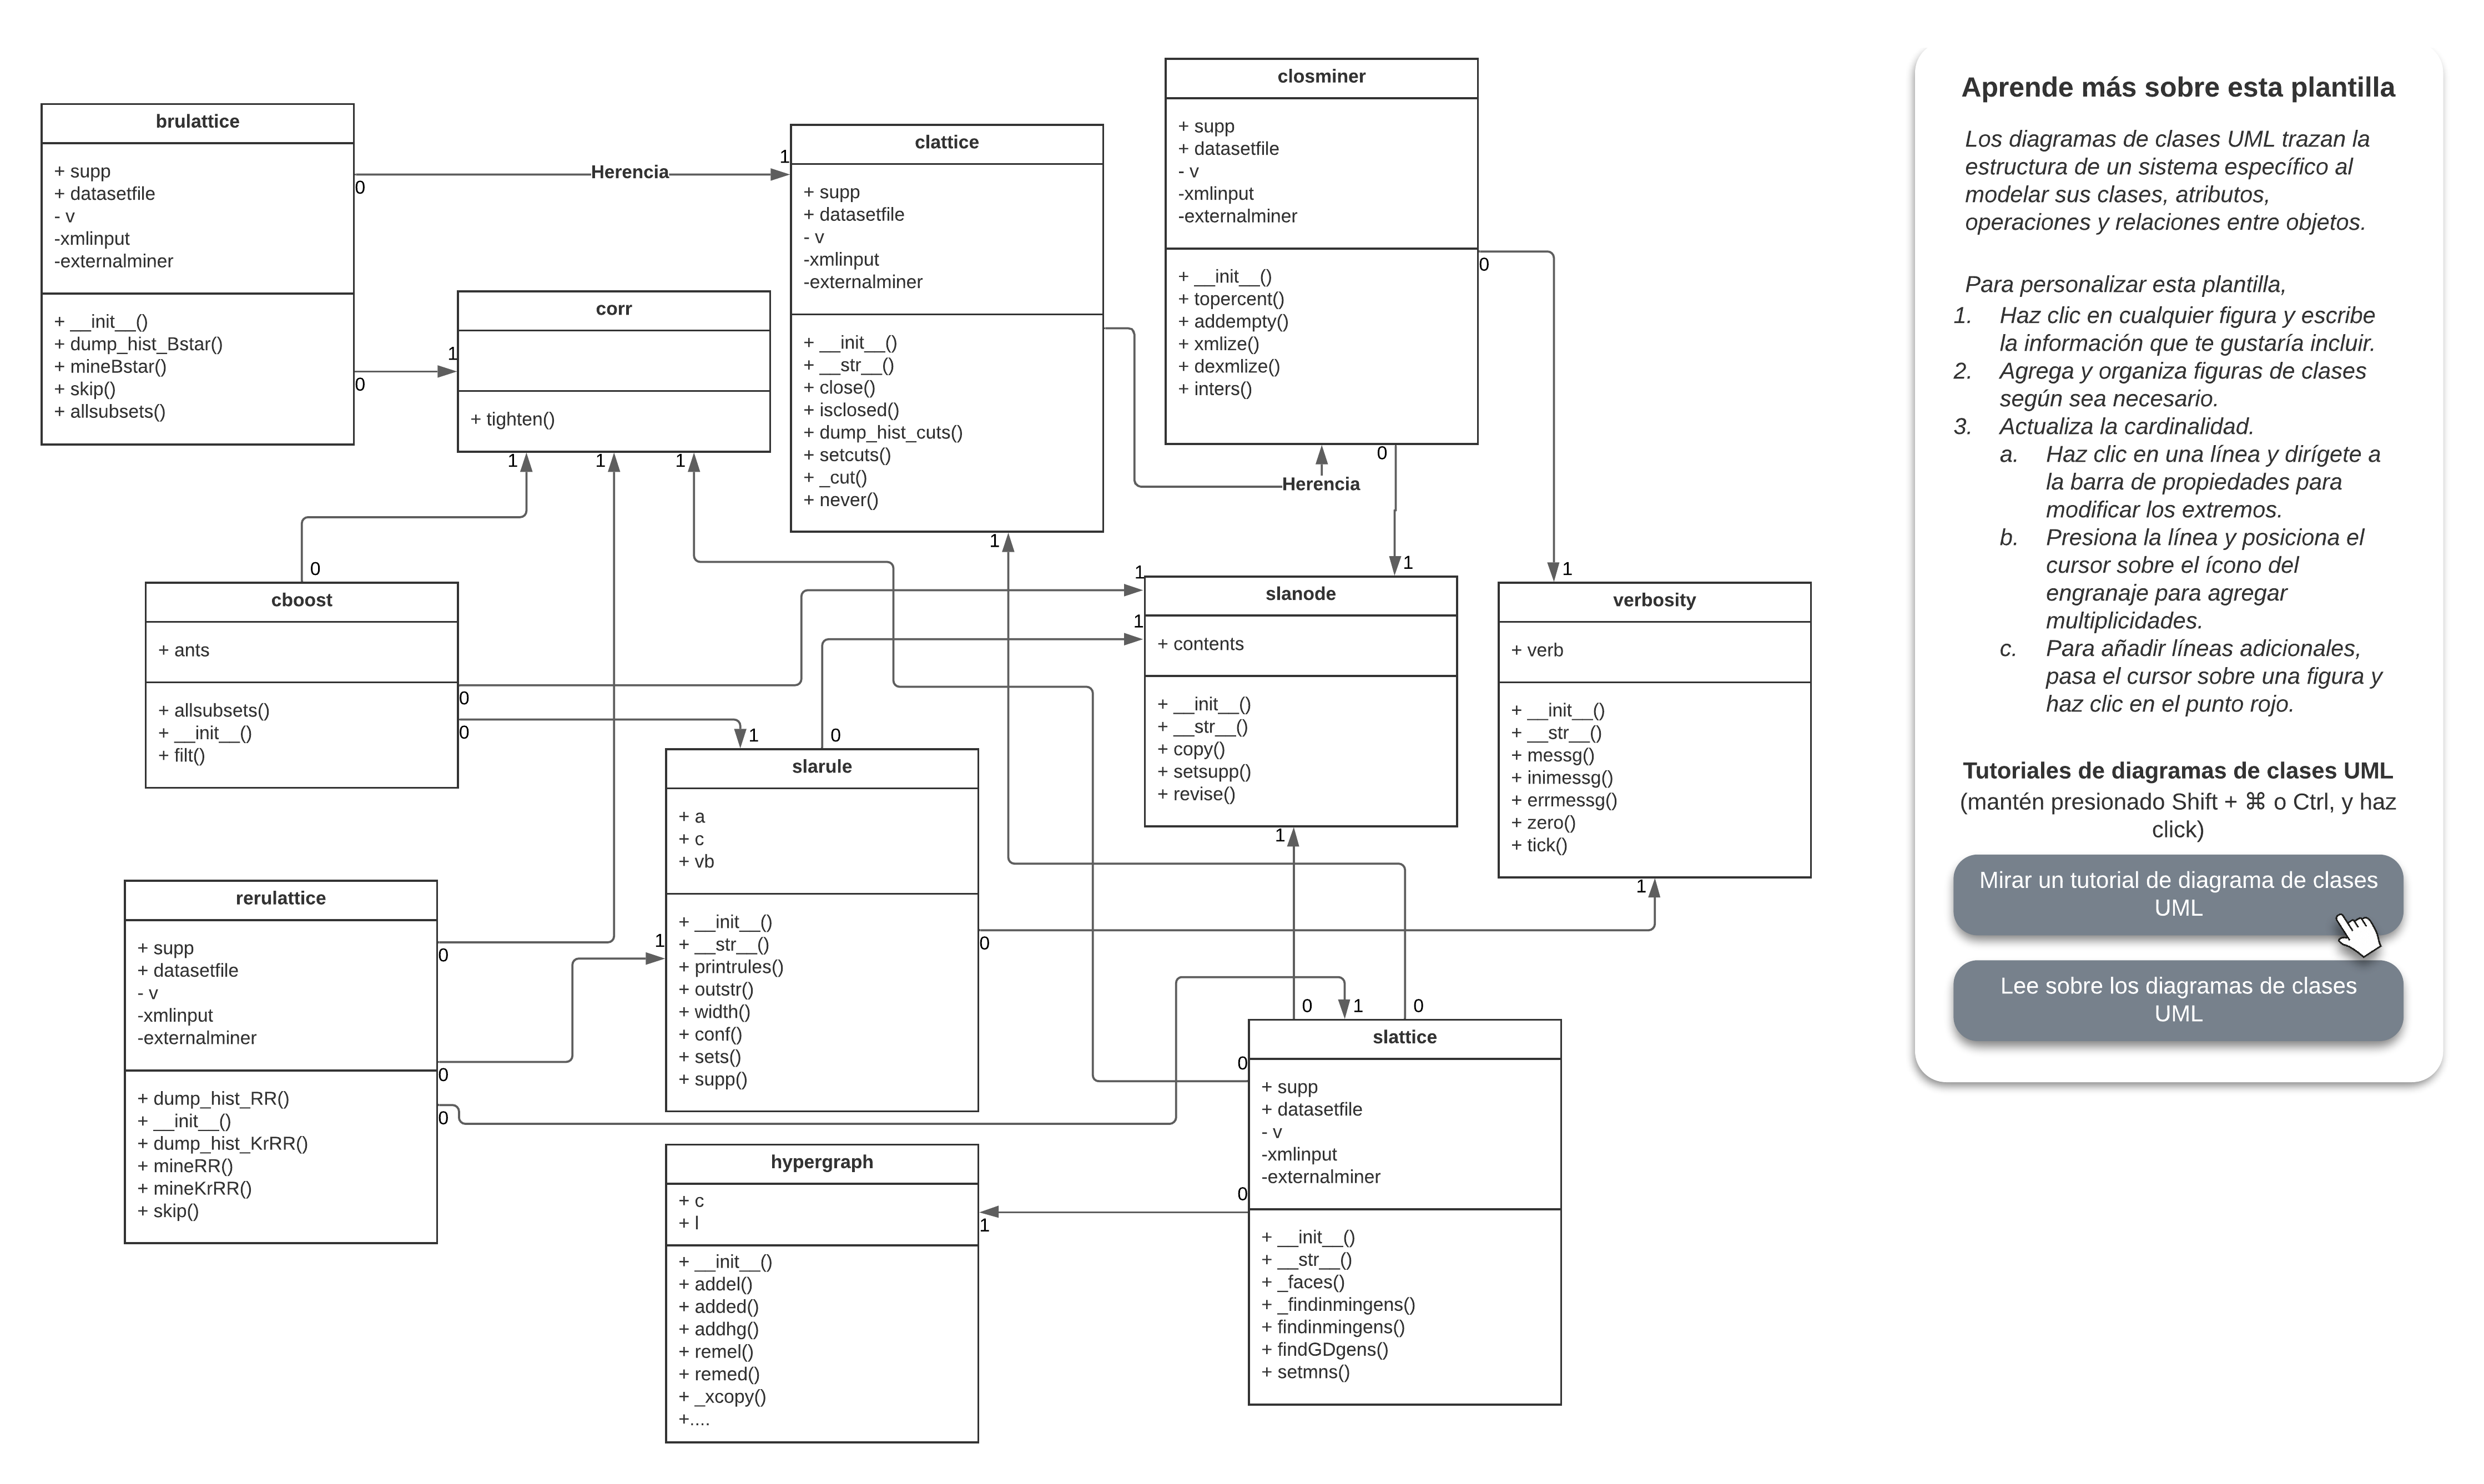
\includegraphics[width=1.45\linewidth]{imagenes/Diagrama en blanco - Clase UML (1).png}
\end{center}
\caption{Diagrama de clases UML Versión Python2}
\label{fig_pro}
\end{figure}



\chapter{\emph{Metaprogramación}}

\section{Conceptos básicos}
En este proyecto se van a utilizar diferentes herramientas relacionadas con la metaprogramación en el entorno de desarrollo.

La metaprogramación consiste en escribir programas que manipulan otros programas, es decir, cuando un programa es capaz de recibir una entrada, modificar el contenido de dicha entrada durante su ejecución y producir como salida otro programa, es un metaprograma.

La metaprogramación se base en estos conceptos principales:

\begin{itemize}
    \item \textbf{Reflexión.- } La capacidad de un programa para observar y modificar su estructura.
    
    Un ejemplo de reflexión seria cuando el código fuente de un programa se compila, se suele perder información sobre la estructura del programa, pero si un sistema permite reflexión, se mantiene dicha estructura como metadatos en el programa generado.
    
    La reflexión se puede descomponer en dos partes:
    
    \begin{enumerate}
        \item \textbf{Introspección.- } La capacidad de un lenguaje de obtener información sobre si mismo.
        
        Un ejemplo de introspección seria java, en java se puede saber hasta nivel del método cuantos atributos, que tipos utiliza, etc.
        \item \textbf{Intercesión.- } La capacidad de modificar el propio comportamiento/ significado de la estructura del programa.
    \end{enumerate}
    
    \item \textbf{Reificación.- } La capacidad de convertir algo abstracto en un dato explícito.
    Ejemplos de reificación serian:
    \begin{itemize}
        \item Crear un tipo de satos para acceder a una posición de memoria
        \item Crear estructuras de datos que representan tipos abstractos de datos
    \end{itemize}
\end{itemize}

En conclusión la metaprogramación es la programación que utiliza los programas como datos y permite modificar su propia estructura. \citep{silva2018metaprogramacion}

\section{Metaprogramación}

David Bleazley en esta charla explica uno de los grandes cambios que existen en Python3 respecto de Python2, la metaprogramación.\citep{David}

En concreto, explica como funcionan los decoradores, la clase \textit{decorators}, los descriptores y las metaclases, estos elementos son usados en este proyecto para mejorar el rendimiento de slatt y reducir a su vez lineas de código.

\subsection{Metaclases}
Una clase es un objeto que se utiliza para crear instancias de nuevos objetos.
Una metaclase está por encima de una clase. Agrupa un conjunto de clases, es decir, podemos tener metainformación sobre clases dentro de una metaclase. Es importante saber que en Python todo es un objeto, incluidas las clases, y cada una de las clases es creada por una metaclase.

\hfill

Por ejemplo:

\begin{verbatim}
def prueba_metaprogramacion():
class Prueba_met:
    pass
return Prueba_met

print(type(prueba_metaprogramacion))
print(type(prueba_metaprogramacion()))
\end{verbatim}

En el primer print la terminal no devuelve: \textit{<class 'function'>}, debido a que $prueba\_metaprogramacion$ pertenece a la clase función. Mientras que en el segundo de los print la terminal devuelve: \textit{<class 'type'>}, debido a que el retorno de $prueba\_metaprogramacion()$ pertenece a la clase tipo.

La clase type es una metaclase. Esta clase se usa para crear otras clases en Python. El constructor de dicha clase se usa para crear clases que pueden crear instacias de dicha clase.

\begin{verbatim}
##El constructor de la clase type tiene esta estructura

type(cls, what, bases=None, dict=None)
El primer parametro es el nombre de la clase
El segundo parametro es una tuple de clases base
El tercer parametro es un diccionario de llaves y valores,
es decir, la implementación de la clase.
\end{verbatim}

Cuando creamos una metaclase que hereda la clase tipo, esta tiene accesso al nombre de la clase, sus padres y todos sus atributos.

\subsection{Clase Type}
$\_\_new\_\_()$ es otro ejemplo de metaprogramación. Crea nuevas instancias de clase y no está vinculado a una instancia de la clase. Este método se llama antes de llamar a $\_\_init\_\_()$. Podemos anular el $\_\_new\_\_()$ de la superclase.
El retorno del método $\_\_new\_\_()$ es la instancia de la clase. Esto es útil cuando queremos modificar la creación de tipos de datos inmutables como las tuplas.

En este proyecto utilizamos este tipo de funcionalidad en la clase decorator.py la cual tiene una clase llamada StructMeta la cual hereda de type e implementa el funcionamiento de el metodo $\_\_new\_\_()$.
\begin{verbatim}
class StructMeta(type):
def __new__(cls, name, bases, clsdict):
    clsobj = super().__new__(cls, name, bases, clsdict)
    sig = make_signature(clsobj._fields)
    setattr(clsobj, '__signature__', sig)
    return clsobj
\end{verbatim}

\subsection{Usos de la Metaprogramación}

\begin{enumerate}
    \item Si queremos comprobar si una clase esta definida correctamente, podemos usar metaclases.
    \item Podemos usar metaclases para generar errores durante la importación de los módulos de la clase.
    \item Podemos usar la metaprogramación si queremos que nuestras clases tengan una convención especifica de métodos y atributos.
    \item Las metaclases se pueden utilizar para modificar el atributo de clase.
    \citep{Farhad}
\end{enumerate}


\chapter{\emph{Hipergrafo y problemas relacionados}}

\section{Conceptos básicos}
En dicho proyecto también se van a tratar elementos como los hipergrafos
y algoritmos con aplicación a estos.

Un hipergrafo H es una familia de subconjuntos (aristas) de un conjunto finito de vértices. Un hipergrafo es simple si ninguno de sus bordes está contenido en ningún otro de sus bordes. Decimos que un hipergrafo está saturado si cada subconjunto del conjunto de vértices está contenido en un borde o contiene un borde de el hipergrafo. \citep{Thomas}

Se toma como algoritmo principal \textit{The algorithm of Berge}, al cual se le añadirán diferentes mejoras analizadas y comprobadas en el paper desarrollado por \citep{JGAA-107} el cual implementa un algoritmo eficiente para la generación transversal de hipergrafos.


% Añadiendo la opción «commandchars=\\\{\}», los caracteres
% \, { y } del archivo fuente se interpretan como código
% LaTeX y puede darse formato al código (manualmente). Hay
% que tener esto en cuenta cuando estos caracteres formen
% parte del código en sí.
%
% Sin esa opción, el fichero de reproduce tal cual.

\begin{center}
% Puede pasar parámetros al comando «VerbatimInput» del
% paquete «fancyvrb». Por ejemplo:


\lstinputlisting[language=python,caption=\textbf{Original Berge Algorithm},frame=bottom]{codigo/berge.py}

\lstinputlisting[language=python,caption=\textbf{Efficient Berge Algorithm},frame=bottom]{codigo/bergeMod.py}


%\codigo[numbers=none,frame=single]{codigo/berge.c}{Original}{11.5cm}

\end{center}

\section{Transversales mínimas de un Hipergrafo}

\newpage
\section{Problemas relacionados con SIMPLE-H-SAT en la teoria de bases de datos}

Siguiendo la lectura del paper \citep{Thomas} en el apartado séptimo habla sobre los diferentes problemas relacionados con el SIMPLE-H-SAT en la teoría de bases de datos.

Inicialmente, habla sobre las bases de datos relaciones y hace una explicación sobre como esta formada una relación, básicamente una
Una relación es una tabla de tuplas distintas de pares de componente que son valores de los dominios de los atributos. Por ejemplo, $U = \{A_0,A_1,...,A_n\}$ es un conjunto de atributos, cada uno de los cuales está asociado a un dominio D. Entonces $D(A_i)$ es el dominio de un atributo $A_i$. 
Entonces una relación sobre U es un subconjunto de $\prod_{i=1}^{n}D(A_i)$, y el los elementos de una relación se denominan tuplas.

El paper también habla sobre las relaciones funcionales, es decir, esas reglas de asociación que nos dan una información de unas variables frente a otras, y lo explica de la siguiente manera:

"Dados los conjuntos $ X, Y $ de atributos, la dependencia funcional (FD) $ X \rightarrow Y $ se mantiene en la relación R si en cada tupla los valores de los atributos en Y están determinados únicamente por los valores de los atributos en X, para tuplas $ t_1 , t_2 \in R \;; t_1 [X] = t_2 [X] $ implica que $ t_1 [Y] = t_2 [Y]: $ Dado que posiblemente todas las tuplas de una relación tienen los mismos valores para algún atributo, el lado izquierdo X de un FD $ X \rightarrow Y $ puede estar vacío. Si $Y \subseteq X$, entonces se llama dependencia funcional trivial."

Y en general, explica como conseguir relaciones funcionales válidas, para ello se tienen que definir diferentes términos.

\begin{itemize}
    \item \textbf{Conjuntos cerrados.-} Son los que no puedes ampliar sin perder soporte. Formalmente hablando, un conjunto $X \subseteq I$ es cerrado si $X=X$, donde $X$ es la clausura de $X$ y se calcula con la $formula :X=\{a \in I |s( X \cup\{a\}) = s(X)\}$
    
    \item \textbf{conjuntos frecuentes.-} $F_\tau=\{X \subseteq I \;|\; s(X) \geq \tau\}$
    \item \textbf{conjuntos frecuentes cerrados.-} $FC_\tau=\{X \in F_\tau \;|\; \forall Z \supset X,s(Z)<s(X)\}$
    \item \textbf{generadores minimales frecuentes.-} $\{X \in F_\tau \;|\; \forall Y \subset X,s(Y)>s(X)\}$
    
\end{itemize}

Con estos elementos definimos si una regla es redundante, sirve para no llenar la base de datos de una misma regla de asociación que se repite durante el tiempo, ocupa espacio innecesario y no ofrece ningún tipo de información valiosa.

Después de la definición de los anteriores conceptos, podemos decir  que una regla de asociación es:

$AR_\tau,_\gamma=\{X\rightarrow Y \;|\; s(X \rightarrow Y)\geq \tau,c(X \rightarrow Y) \geq \gamma\}$, siendo $\tau$ y $\gamma$ umbrales de soporte y confianza respectivamente.

También podemos definir la reglas representativas como:

$RR_\tau,_\gamma=\{r \in AR_\tau,_\gamma \;|\; \nexists \; r′ \in AR_\tau, \;|\; \gamma\{r\}$ tal que $r \in C(r′)\}$ \citep{UC}

Con esta definición de regla representativa no redundante podemos conseguir una cantidad de reglas de asociación menor con un mismo valor de contenido, es decir, nos ahorraríamos mucho espacio en una base de datos gracias a esta definición de regla representativa.

\section{Axiomas de Armstrong}

Los Axiomas de Armstrong son en su esencia reglas de inferencia mencionadas anteriormente.
Estas reglas permiten deducir todas las dependencias funcionales que tienen
lugar entre un conjunto dado de atributos $A=\{A_1,A_2,...,A_n\}$ , como consecuencia de las dependencias dadas, es decir, se deducen todas las dependencias que se asumen ciertas a partir del conocimiento del problema.

\subsection{Ejemplo de axiomas de Armstrong}
Tenemos una relación R con tres atributos (A,B,C), ahora, después de realizar la función de dependencias, nos devuelve las dos siguientes reglas $F = \{A \rightarrow B , \; B \rightarrow C\}$, con estas dos reglas podemos inferir el conjunto completo de funciones de dependencias que serian: $\{ A \rightarrow C , A \rightarrow A , B \rightarrow B , C \rightarrow C ,\}$.

Ahora tenemos un set F con las dos reglas de dependencias y un superset $F^+$ el cual es un set de funciones lógicamente inferidas de F. A continuación, muestro una tabla de la relación entre el numero de atributos combinados y las posibles keys que podemos elegir.

\begin{table}[h]
\begin{tabular}{|l|l|l|l|}
\hline
                               & \multicolumn{3}{l|}{\# de atributos combinados} \\ \hline
\multirow{4}{*}{Posibles keys} & 1              & 2               & 3                \\ \cline{2-4} 
                               & A              & AB              & ABC              \\ \cline{2-4} 
                               & B              & AC              &                  \\ \cline{2-4} 
                               & C              & BC              &                  \\ \hline
Total                          & 3              & 3               & 1                \\ \hline
\end{tabular}
\end{table}

En este caso es sencillo debido a que únicamente tenemos 3 atributos posibles, pero en el caso que por ejemplo tengamos un numero elevado de ellos A = 100 se puede utilizar una formula matemática que calcula el numero de posibilidades $\frac{n!}{(n-r)! (r)!}$ donde r es número total de atributos y n cuantos atributos por key tenemos.

Una vez tenemos esto necesitamos un mecanismo que nos permita conocer si las reglas de dependencia están dentro o fuera del $F^+$, es entonces cuando utilizamos los axiomas de Armstrong.

Para ello primero definiré que es un axioma, según la tercera definición del diccionario, un axioma es una proposición que se asume sin prueba, con el fin de estudiar las consecuencias que se derivan de ella. Los axiomas de armstrong tienen tres acciones reflexividad, aumentatividad y transitividad, que son en términos matemáticos definidas de la siguiente manera:

\begin{enumerate}
    \item \textbf{Reflexividad} $\forall X , X \rightarrow X $ $ex. (ABC \rightarrow AB)$
    
    \item \textbf{Aumentatividad} $\{ X \rightarrow Y , Z \supseteq X \} \Rightarrow Z \rightarrow Y  $ $ex. (AC \rightarrow CB)$
    
    \item \textbf{Transitividad} $ \{ X\rightarrow Z , Z \rightarrow Y \} \Rightarrow X \rightarrow Y $ $ex. (A \rightarrow B , B \rightarrow C) \Rightarrow (A \rightarrow C)$
\end{enumerate}

Si tenemos en $F^+$ un set de todas las funciones con dependencias las cuales hemos inferido de F, si aplicamos las acciones de armstrong a F no vamos a encontrar ningún set de funciones con dependencias fuera de F solo podremos encontrar estas funciones dentro de F.

otro aspecto de los axiomas de armstrong es que es completo esto quiere decir que si aplicamos acciones de armstrong a F vamos a encontrar todas las funciones con dependencias existentes en dicho set.




\chapter{\emph{KD Trees}}

\section{Conceptos básicos}

Un KD Tree (también conocido como K-Dimensional Tree) es un árbol de búsqueda binario donde los datos en cada nodo son un punto k-dimensional en el espacio. Básicamente, es una estructura de datos que utiliza una partición en el espacio para organizar puntos en un espacio K-Dimensional.

\begin{enumerate}
    \item Cada nodo tiene como clave multidimensional un vector de tamaño k
que contiene los valores de las k claves unidimensionales y tiene asociado un discriminante con valor entero entre 1 y k.
    \item Para cada nodo con clave multidimensional x y discriminante j se
cumple que cualquier nodo del subárbol izquierdo con clave multidimensional y cumple que su n-ésima componente es menor que la n-ésima componente de x, es decir (yn < xn ). Para el subárbol derecho se cumple que la n-ésima componente de la clave multidimensional z de cualquier nodo de este subárbol es mayor que la n-ésima componente de la clave x, es decir (zn > xn ).
    \item La raíz del kd-tree tiene profundidad 0 y discriminante 1. Cualquier
nodo a una profundidad p tiene discriminante de valor: (p mod k) + 1.
\citep{marti2010copy}
\end{enumerate}

Otra de las aplicaciones es la de representar un conjunto de puntos y la consulta más frecuente sobre este conjunto es la de localizar el punto o puntos más cercanos a uno dado. Esta consulta se conoce con el nombre de búsqueda del vecino más cercano.

\section{Implementación en Reglas de Asociación}

Los kd-trees son frecuentemente utilizados en bases de datos para satisfacer consultas que incluyan valores de varios campos. Esto se puede extrapolar a las reglas de asociación, ya que se podrían realizar consultas como se ha explicado en el ejemplo introductorio de reglas de asociación.

\hspace{0.5mm}

Una consulta podría ser por ejemplo, saber todos los registros de personas que compren pan, leche y huevos, y además tengan entre 25 y 45 años, y que vivan en España, todo esto se podría realizar en una única consulta utilizando los \textit{KD trees} como algoritmo de búsqueda ya que permite realizar diferentes consultas simultaneas, en lugar del algoritmo \textit{apriori} actualmente utilizado, en el que al añadir múltiples consultas, su coste computacional hace que no tenga sentido dicho calculo, debido a su lento proceso.

\newpage
\section{Ejemplo gráfico KD Tree}

\hfill

Ejemplo gráfico de un KD-tree para el siguiente ItemSet:

\textbf{{(3,6),(17,15),(13,15),(6,12),(9,1),(2,7),(10,19)}}

\hfill

\begin{figure}[h]
\begin{center}
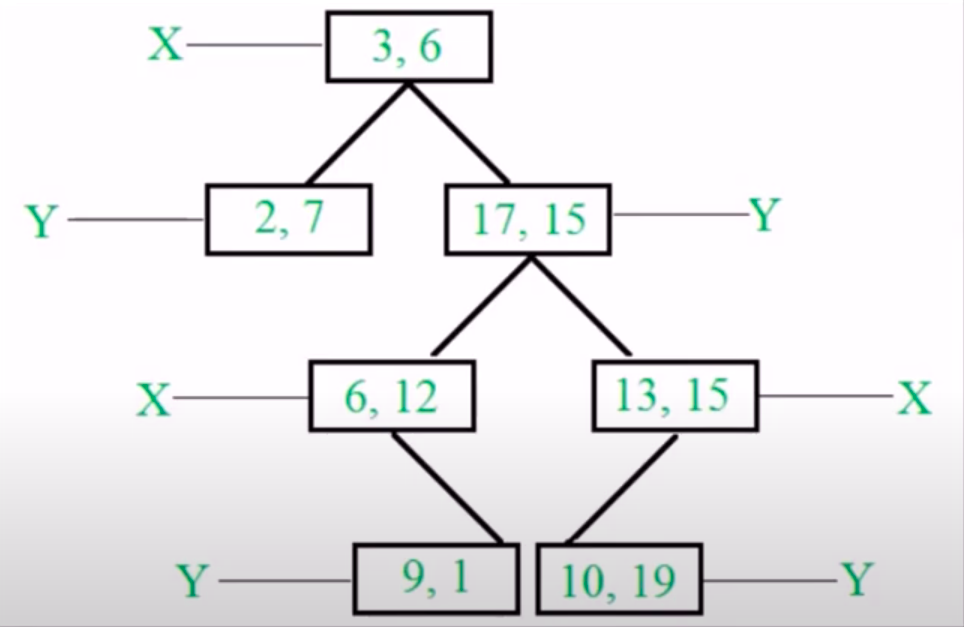
\includegraphics[width=.4\linewidth]{imagenes/kdtree1.png}
\end{center}
\caption{Árbol del ItemSet}
\label{arbol_kd}
\end{figure}

\begin{figure}[h]
\begin{center}
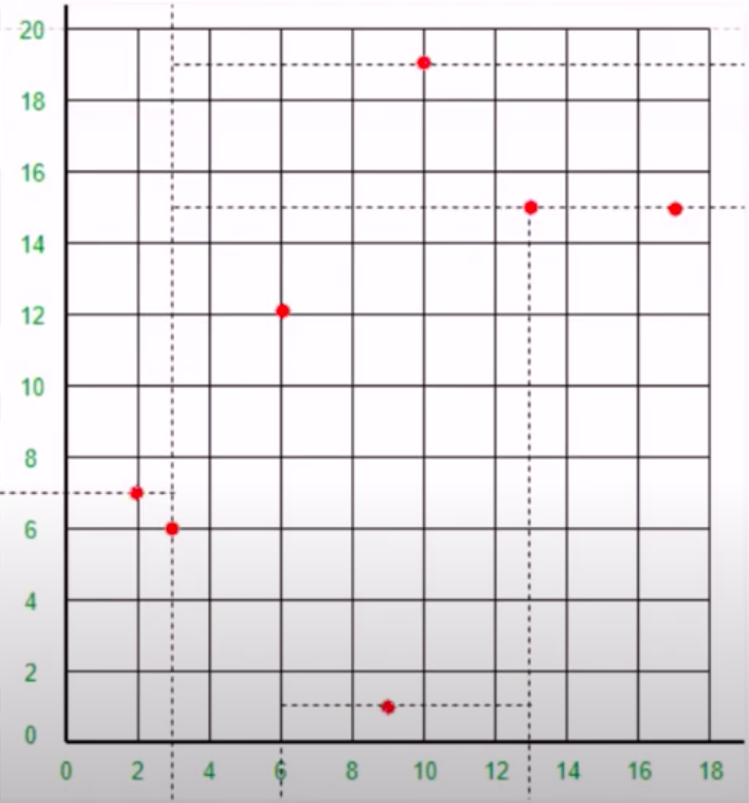
\includegraphics[width=.4\linewidth]{imagenes/kdtree2.png}
\end{center}
\caption{Gráfica del ItemSet}
\label{grafica_kd}
\end{figure}

Desde un punto de vista geométrico como se ve en la Ilustración \ref{arbol_kd}, cada nodo del kd tree hace una partición del plano en dos “subplanos”. En la Ilustración \ref{grafica_kd} todos los puntos en el “subplano” de la izquierda corresponden al subárbol izquierdo del nodo raíz, y los que quedan a la derecha son los puntos del subárbol derecho.


\chapter{\emph{Desarrollo Software}}
En este aparatado del proyecto se muestran que cambios han sido necesarios en el código para la correcta ejecución de Slatt pasando todo su código de python2 a python3, los test necesarios para su correcto funcionamiento y además se explica que mejoras se han llevado a cabo tanto de rendimiento, como en la reducción del número de lineas de código.

\section{Test unitarios}

En esta sección se especifica como se realizan los test unitarios, para comprobar si las dos versiones del código mantienen la misma funcionalidad basándose en la salida de estos test.

\hfill

\lstinputlisting[language=bash,caption=\textbf{Makefile},frame=bottom]{codigo/makefile}

Utilizando este \textbf{makefile} se realiza una ejecución simultanea de ambas versiones, guardando dicha salida en un fichero.txt y a continuación, se hace un \textbf{diff} entre los dos archivos, en el caso en el que el \textbf{diff} devuelva un archivo vacío, sabremos que las dos versiones tienen la misma funcionalidad.

\section{Mejoras del código}
En esta sección se va a discutir cuales han sido los cambios y mejoras en cada una de las clases que se han modificado en el código:

\subsection{Diferencias entre python2 y python3}

En la actualidad, existen dos tipos de versiones de python, las cuales son 2.x en la que está inicialmente escrita Slatt y 3.x en la cual se ha estado desarrollado este proyecto.

Las principales diferencias que he encontrado en el proyecto han sido las siguientes \citep{diferencias}:

\begin{enumerate}
    \item \textbf{Sentencia print}
    
    Esta posiblemente sea la diferencia que más veces ha aparecido en el proyecto, ya que en prácticamente todas y cada una de las clases aparece algún print en el main o en algún método de la propia clase.
    Se soluciona de una manera muy sencilla, añadiendo el el argumento de la sentencia print dos paréntesis. (print \textbf{x} --> print( \textbf{x} ))
    
    \item \textbf{Comparación de tipos}
    
    En \textbf{pyhton2} se permiten las comparaciones entre objetos de distintos tipos, mientras que en \textbf{python3} nos lanza una excepción del tipo \textit{TypeError}, esto a sido necesario tenerlo en cuanta en el código porque había bastantes comparaciones de tipos distintos a lo largo del código en clase como brulattice.py o closminer.py.
    
    \item \textbf{División de números enteros}
    
    En \textbf{python2} la división entre números enteros da un numero entero y si quieres conseguir un resultado con decimales necesitas que uno de los dos números de la operación tengan un decimal, en este caso en \textbf{python3} se hace mediante un truncado de la división usando el // en lugar de /.
    
    \item \textbf{Iterar un diccionario}
    
    La ultima diferencia que se ha detectado en código a la hora de hacer la reescritura a \textbf{python3} a sido la iteración de diccionarios ya que en \textbf{python2} se pueden iterar los elementos clave-valor de un diccionario con el método \textit{iteritems()} o \textit{items()}, mientras que en python3 únicamente se puede usar el segundo de estos dos métodos, ya que con el primero de ellos se produce una excepción de tipo \textit{AttributeError}.
    A su vez, los métodos \textit{iterkeys()} e \textit{itervalues()} para iterar las claves y los valores de un diccionario respectivamente no existen en Python 3. En su lugar tenemos que usar los métodos \textit{keys()} y \textit{values()}. Estos métodos tanto \textit{keys()}, \textit{values()} como items() se han visto afectados en clases como brulattice.py o cboost.py
    
\end{enumerate}



\begin{itemize}

\item \textbf{brulattice.py}

\item \textbf{cboost.py}

En la clase cboost.py inicialmente he modificado el método allsubsets para que sea mas corto y enfiente utilizando la libreria de combinations procedente de itertools la cual me permite realizar un for anidado de una manera más eficiente y con un número de lineas reducido.
Tambein 

\item \textbf{clattice.py}

\item \textbf{closminer.py}

\item \textbf{corr.py}

\item \textbf{decorator.py}

La clase decorator.py es una nueva clase implementada para \textbf{python3} la cual nos permite utilizar diferentes funcionalidades de la metaprogramación mencionadas anteriormente, como es la creación de constructores mediante una simple linea de código gracias a las clase Structure  y la variable \_fields o incluso introducir partes del código (funciones, métodos) con otra variable llamada \_processing.

También se introducen un método que nos permite saber quienes son las clases padre de una clase u objeto, gracias al modulo \textit{Signature} de la clase inspect.py.

\item \textbf{hypergraph.py}

En la clase hypergraph se realiza una herencia de la clase Structure, para eliminar su \_\_init\_\_ sustituyéndolo por la variable \_fields y con ello reducir el número de lineas de código.
También se ha diseñado un patrón decorator el cual sustituye la mayoría de las funciones que se encuentran en dicha clase:  \textbf{[addel,added,addhg,remel,remed]}, este cambio se llevó a cabo debido a que se vio un claro patrón de repetición en todas las funciones de la clase, el patrón es el siguiente:

\begin{verbatim}
        def decorator(self,a1,a2,a3,a4,a5):
        if a1:
            a1()
        for e in a2:
            a3(e)
        if a4:
            a4(a2)
        if a5:
            a5()
\end{verbatim}

Con este patrón se consigue resumir todas y cada una de las funciones de la clase en una única linea de código, para ello tuve que usar funcionalidades como \textit{lambda} la cual permite generar una función dentro del patrón decorator. (\# lineas antes = 142, \# lineas después = 134)

\item \textbf{rerulattice.py}

\item \textbf{slanode.py}

En esta clase slanody.py se ha eliminado la clase \textit{auxitset} con todos sus métodos, introduciéndola dentro de la propia clase \textit{slanode}, en concreto se han introducido los dos métodos \textit{str2node} y \textit{set2node} en la clase \textit{slanode} y también se ha creado el \_\_init\_\_ de \textit{auxitset} y \textit{slanode} con un solo método llamado \_\_new\_\_ que introduce como parámetros los atributos de la clase y los inicializa sin ser necesario usar una clase auxiliar.

\item \textbf{slarule.py}

En esta otra clase se añade también al herencia de la clase decorator para poder minimizar la creación del constructor \_\_init\_\_ , se eliminan todas la ocurrencias de igualdad con 0, ya que en este caso siempre es verdadero y por lo tanto, las reglas if x = 0 son inutiles un ejemplo de ello seria:

\begin{verbatim}
    if self.an.supp == 0:
        self.confval = float(self.cn.supp)/self.an.supp
        
    #### Se sustituye por: #####
    
    if not self.an.supp:
        self.confval = float(self.cn.supp)/self.an.supp
\end{verbatim}

Con este simple cambio se genera un pequeña mejora en el rendimineto del programa y a su vez facilita la compresión del mismo.

\item \textbf{slattice.py}
    
\item \textbf{verbosity.py}

En esta clase se añade una herencia de la clase decorator.py previamente analizada, verbosity utiliza una de las clases de decorator llamada Structure la cual permite eliminar el \_\_init\_\_ de la clase añadiendo una unica variable llamada \_fields, en la cual se definen cada uno de los parametros definidos en el \_\_init\_\_, tanto argumentos como los propios atributos de la clase.

En código se ve así:
\begin{verbatim}
        def __init__(self,verb=True):
        """
        verbosity;
        lim and count for the progress-reporting ticks;
        """
        self.verb = verb
        self.lim = 0
        self.count = 0
        
        #### Se sustituye por: #####
        
        _fields = [('verb', True), ('lim', 0), ('count', 0)]
\end{verbatim}

Con este cambio conseguimos una mejora en cuanto al número de lineas y simplicidad de código enorme, ya que realizar el constructor de la clase antes nos costaba 7 lineas donde ahora lo podemos conseguir en una. Por lo demás, los demás cambios han sido simplemente en la sintaxis ya que python2 y python3 tienen diferencias en el lexico. (\# lineas antes = 47, \# lineas después = 35)
\end{itemize}

\chapter{\emph{Conclusiones}}

% Indique aquí el fichero .bib que contenga su bibliografía.
\bibliography{refs}

\end{document}
